\documentclass[11pt,a4paper,fleqn]{article}

\usepackage[margin=1in]{geometry}
\usepackage{amsmath,amssymb,amsfonts}
\setlength{\mathindent}{1.5em}
\usepackage{algorithmic}
\usepackage{algorithm}
\usepackage{graphicx}
\usepackage{textcomp}
\usepackage{xcolor}
\usepackage{booktabs}
\usepackage{hyperref}
\usepackage{microtype}
\usepackage{subcaption}
\usepackage{url}
\usepackage{setspace}
\usepackage[running]{lineno}
\usepackage[authoryear,round]{natbib}

\setstretch{1.15}
\linenumbers

\hypersetup{
    colorlinks=true,
    linkcolor=blue,
    filecolor=magenta,      
    urlcolor=blue,
    citecolor=blue
}

\begin{document}
\pagestyle{plain}
\thispagestyle{plain}

% =========================================================================
% FRONT MATTER (Journal of Hydroinformatics - IWA Publishing / OUP Format)
% =========================================================================

\begin{singlespace}
\noindent{\Large \textbf{Physics-anchored hybrid hydrological modeling using satellite Earth observation for monthly volumetric flood risk and extreme generalization in the Lower Indus Basin, Pakistan}}\\[1.5em]

\noindent Mirza Muhammad Muzzamil$^{1*}$\\[0.8em]

\noindent $^1$Department of Computer and Information Systems Engineering (CISE), NED University of Engineering and Technology, University Road, Karachi 75270, Sindh, Pakistan\\[1.2em]

\noindent \textbf{*Corresponding author:}\\
\noindent Mirza Muhammad Muzzamil\\
\noindent Department of Computer and Information Systems Engineering (CISE), NED University of Engineering and Technology, Karachi 75270, Pakistan\\
\noindent E-mail address: \href{mailto:mirzamuzzamil@neduet.edu.pk}{mirzamuzzamil@neduet.edu.pk}\\
\noindent ORCID iD: \href{https://orcid.org/0000-0001-5258-8959}{0000-0001-5258-8959}\\[1.5em]

\noindent \textbf{Highlights}
\begin{itemize}
    \item A multi-decadal (2000--2024, $N=300$) physics-anchored hybrid framework is developed for the Lower Indus Basin ($140,914\text{ km}^2$).
    \item Antecedent memory is strictly formulated as lagged storage ($API_t = \gamma P_{t-1} + \gamma^2 P_{t-2}$), eliminating precipitation double-counting.
    \item Non-negative regularized linear water-balance base model anchors non-linear residual decision tree ensembles.
    \item Achieves superior out-of-distribution generalization during the unseen 2022 Pakistan Mega-Flood ($\text{KGE} = 0.812$, $FHV = -4.0\%$).
    \item Restricts out-of-sample peak underestimation compared to purely unconstrained machine learning ($FHV = -13.3\%$).
\end{itemize}
\vspace{1.0em}

\noindent \textbf{Abstract}\\
Accurate monthly streamflow and volumetric flood risk forecasting in heavily managed, low-gradient alluvial basins remains a fundamental challenge in hydroinformatics due to complex hydrometeorological non-stationarity, intensive canal diversions, transboundary upstream inflows, and in-situ observational scarcity. While modern machine learning models capture complex non-linear rainfall-runoff processes, unconstrained architectures frequently suffer from physical inconsistency and severe peak flow dampening under out-of-distribution climate extremes. We present a Physics-Anchored Water-Balance Hybrid Hydroinformatics Framework (PG-MCH) for the Lower Indus Basin within Sindh Province, Pakistan ($140,914\text{ km}^2$). The model couples a non-negative, L2-regularized linear water-balance baseline with multi-sensor residual gradient boosted decision trees and dual physical mass conservation bounding operators. The framework ingests multi-decadal satellite Earth observation streams extracted via Google Earth Engine across 2000--2024 ($N=300$ continuous monthly observations), comprising CHIRPS v2.0 precipitation, ERA5-Land temperature and evaporation, SMAP root-zone soil moisture, and GRACE terrestrial water storage anomalies, alongside gauged upstream transboundary telemetry at Guddu Barrage. Catchment antecedent moisture memory is formulated strictly as lagged storage ($API_t = \gamma P_{t-1} + \gamma^2 P_{t-2}$), guaranteeing that current precipitation is counted exactly once within a rigorous mass-conservation envelope ($W_{\text{total}} = P(t) + Q_{\text{inflow}}(t) + API_t$). Model calibration is established over a 20-year baseline record (2000--2019, $N=240$ months) and stress-tested against the catastrophic 2022 Pakistan Mega-Flood (+350\% monsoon anomaly) and a 2023--2024 non-stationary validation period ($N=60$ out-of-sample months). During the unseen 2022 Mega-Flood holdout, PG-MCH achieved a Kling-Gupta Efficiency (KGE) of 0.812 and restricted peak flow underestimation bias ($FHV$) to $-4.0\%$, significantly outperforming unconstrained gradient boosting ($FHV = -13.3\%$) and Random Forest ($FHV = -7.0\%$). Across the 2020--2024 out-of-sample period, PG-MCH achieved $\text{KGE} = 0.895\ [95\%\text{ CI: } 0.73, 0.93]$, $\text{NSE} = 0.838$, and $\text{RMSE} = 11.78\text{ mm/month}$. Systematic ablations confirm that anchoring residual machine learning to physical water-balance baselines prevents peak collapse and guarantees robust extreme generalization.\\[1.2em]

\noindent \textbf{Keywords:} Physics-guided machine learning, Hydroinformatics, Google Earth Engine, Indus River Basin, Flood generalization, Water balance\\[1.5em]

\end{singlespace}

\newpage

% =========================================================================
% MAIN TEXT
% =========================================================================

\section{Introduction}
The Indus River Basin is one of the world's most critical and climate-vulnerable transboundary river basins, sustaining over 230 million people and supporting the largest contiguous surface irrigation network on Earth---the Indus Basin Irrigation System (IBIS) \citep{immerzeel2020importance, young2019pakistan}. The lower reach of the basin, located within Sindh Province, Pakistan, represents an extreme hydraulic, ecological, and socioeconomic bottleneck. Across this reach, the Indus River flows across low-gradient alluvial floodplains before discharging into the northern Arabian Sea through the Indus Delta \citep{hashmi2022hydrodynamic, inam2007geographic}.

In recent decades, intensifying climate extremes have aggravated hydro-climatic volatility across South Asia. In July--August 2022, anomalous atmospheric monsoon depressions produced unprecedented torrential downpours across Pakistan, with Sindh Province receiving over 350\% of its 30-year climatological monsoon precipitation \citep{nanditha20232022, syed2022analysis, wwa2022pakistan}. Synthetic Aperture Radar (SAR) remote sensing confirmed that over one-third of the province's surface area was inundated \citep{tian2023satellite}, resulting in massive socioeconomic loss and threatening catastrophic structural breaches at strategic barrage infrastructure (Guddu, Sukkur, and Kotri Barrages) and regional retention reservoirs (Manchar Lake). Conversely, the basin frequently experiences severe dry-season agricultural droughts, groundwater depletion, and pre-monsoon heatwaves \citep{biemans2016future, rodell2018emerging}.

\subsection{Hydroinformatics challenges in managed alluvial basins}
Developing reliable monthly volumetric streamflow and flood risk forecasting in large alluvial basins involves two core challenges:
\begin{enumerate}
    \item \textbf{Limitations of conceptual hydrological models:} Conceptual rainfall-runoff models (such as GR4J and SAC-SMA) rely on calibrated parameter sets that assume climatic stationarity \citep{frame2022post, gupta2009decomposition, perrin2003improvement}. Under unprecedented climatic extremes, these empirical structures degrade significantly. Moreover, integrating high-dimensional gridded satellite Earth observations into lumped or semi-distributed conceptual models remains challenging.
    \item \textbf{Limitations of purely data-driven machine learning:} Machine learning models (e.g., Random Forests, Gradient Boosted Decision Trees, Long Short-Term Memory networks) excel at discovering complex non-linear patterns from multi-sensor data \citep{kratzert2018rainfall, kratzert2019towards, nearing2024global}. However, unconstrained black-box models frequently produce unphysical predictions (such as negative streamflow) and suffer from severe conditional variance shrinkage when tested on out-of-distribution (OOD) extremes \citep{jia2021physics, karpatne2017physics, read2019process}. Because decision tree ensembles partition feature spaces with orthogonal decision boundaries, they cannot extrapolate beyond historic training maxima, resulting in systematic peak flow underestimation.
\end{enumerate}

\subsection{Research objectives and novelty}
To address these limitations, this study presents a **Physics-Anchored Water-Balance Hybrid Hydroinformatics Framework (PG-MCH)** that reconciles physical mass conservation with the non-linear predictive capacity of ensemble machine learning. The specific objectives and novel contributions are:
\begin{enumerate}
    \item \textbf{Physics-guided hybrid architecture:} Formulating a multi-tier framework combining a Non-Negative Least Squares (NNLS) physical water-balance baseline with a residual Gradient Boosted Decision Tree (GBDT) ensemble.
    \item \textbf{Strict mass conservation without double-counting:} Reformulating antecedent catchment wetness strictly as lagged storage memory ($API_t = \gamma P_{t-1} + \gamma^2 P_{t-2}$), ensuring that current precipitation is counted exactly once within a rigorous upper mass envelope ($W_{\text{total}} = P(t) + Q_{\text{inflow}}(t) + API_t$).
    \item \textbf{Multi-decadal baseline and extreme holdout protocol:} Calibrating the framework on a 20-year multi-decadal record (2000--2019, $N=240$ months) and stress-testing under a zero-shot holdout protocol against the catastrophic 2022 Pakistan Mega-Flood and 2023--2024 recovery period ($N=60$ out-of-sample months).
    \item \textbf{Physical ablation analysis & uncertainty quantification:} Conducting systematic multi-regime ablations and non-parametric Moving Block Bootstrap (MBB, $B=1,000$) uncertainty quantification to demonstrate physical consistency across flood and drought phases.
\end{enumerate}

\section{Study Area and Hydro-Meteorological Datasets}

\subsection{Geographical and hydraulic context of the Lower Indus Basin}
The study domain encompasses the entire administrative boundary of Sindh Province, Pakistan, covering an area of $140,914\text{ km}^2$ located between latitudes $23.4^\circ\text{N}$--$29.0^\circ\text{N}$ and longitudes $66.4^\circ\text{E}$--$71.4^\circ\text{E}$ (\textbf{Fig. 1}). The hydrological regime is defined by the mainstem Indus River, which enters northern Sindh at Guddu Barrage, traverses southwards past Sukkur Barrage and Kotri Barrage, and discharges into the Arabian Sea via the Indus Delta. The hydraulic slope across the alluvial plains is exceptionally flat ($< 0.8^\circ$), creating prolonged water retention and extensive inundation during peak monsoon surges \citep{hashmi2022hydrodynamic, inam2007geographic}.

\begin{figure}[htbp]
\centering
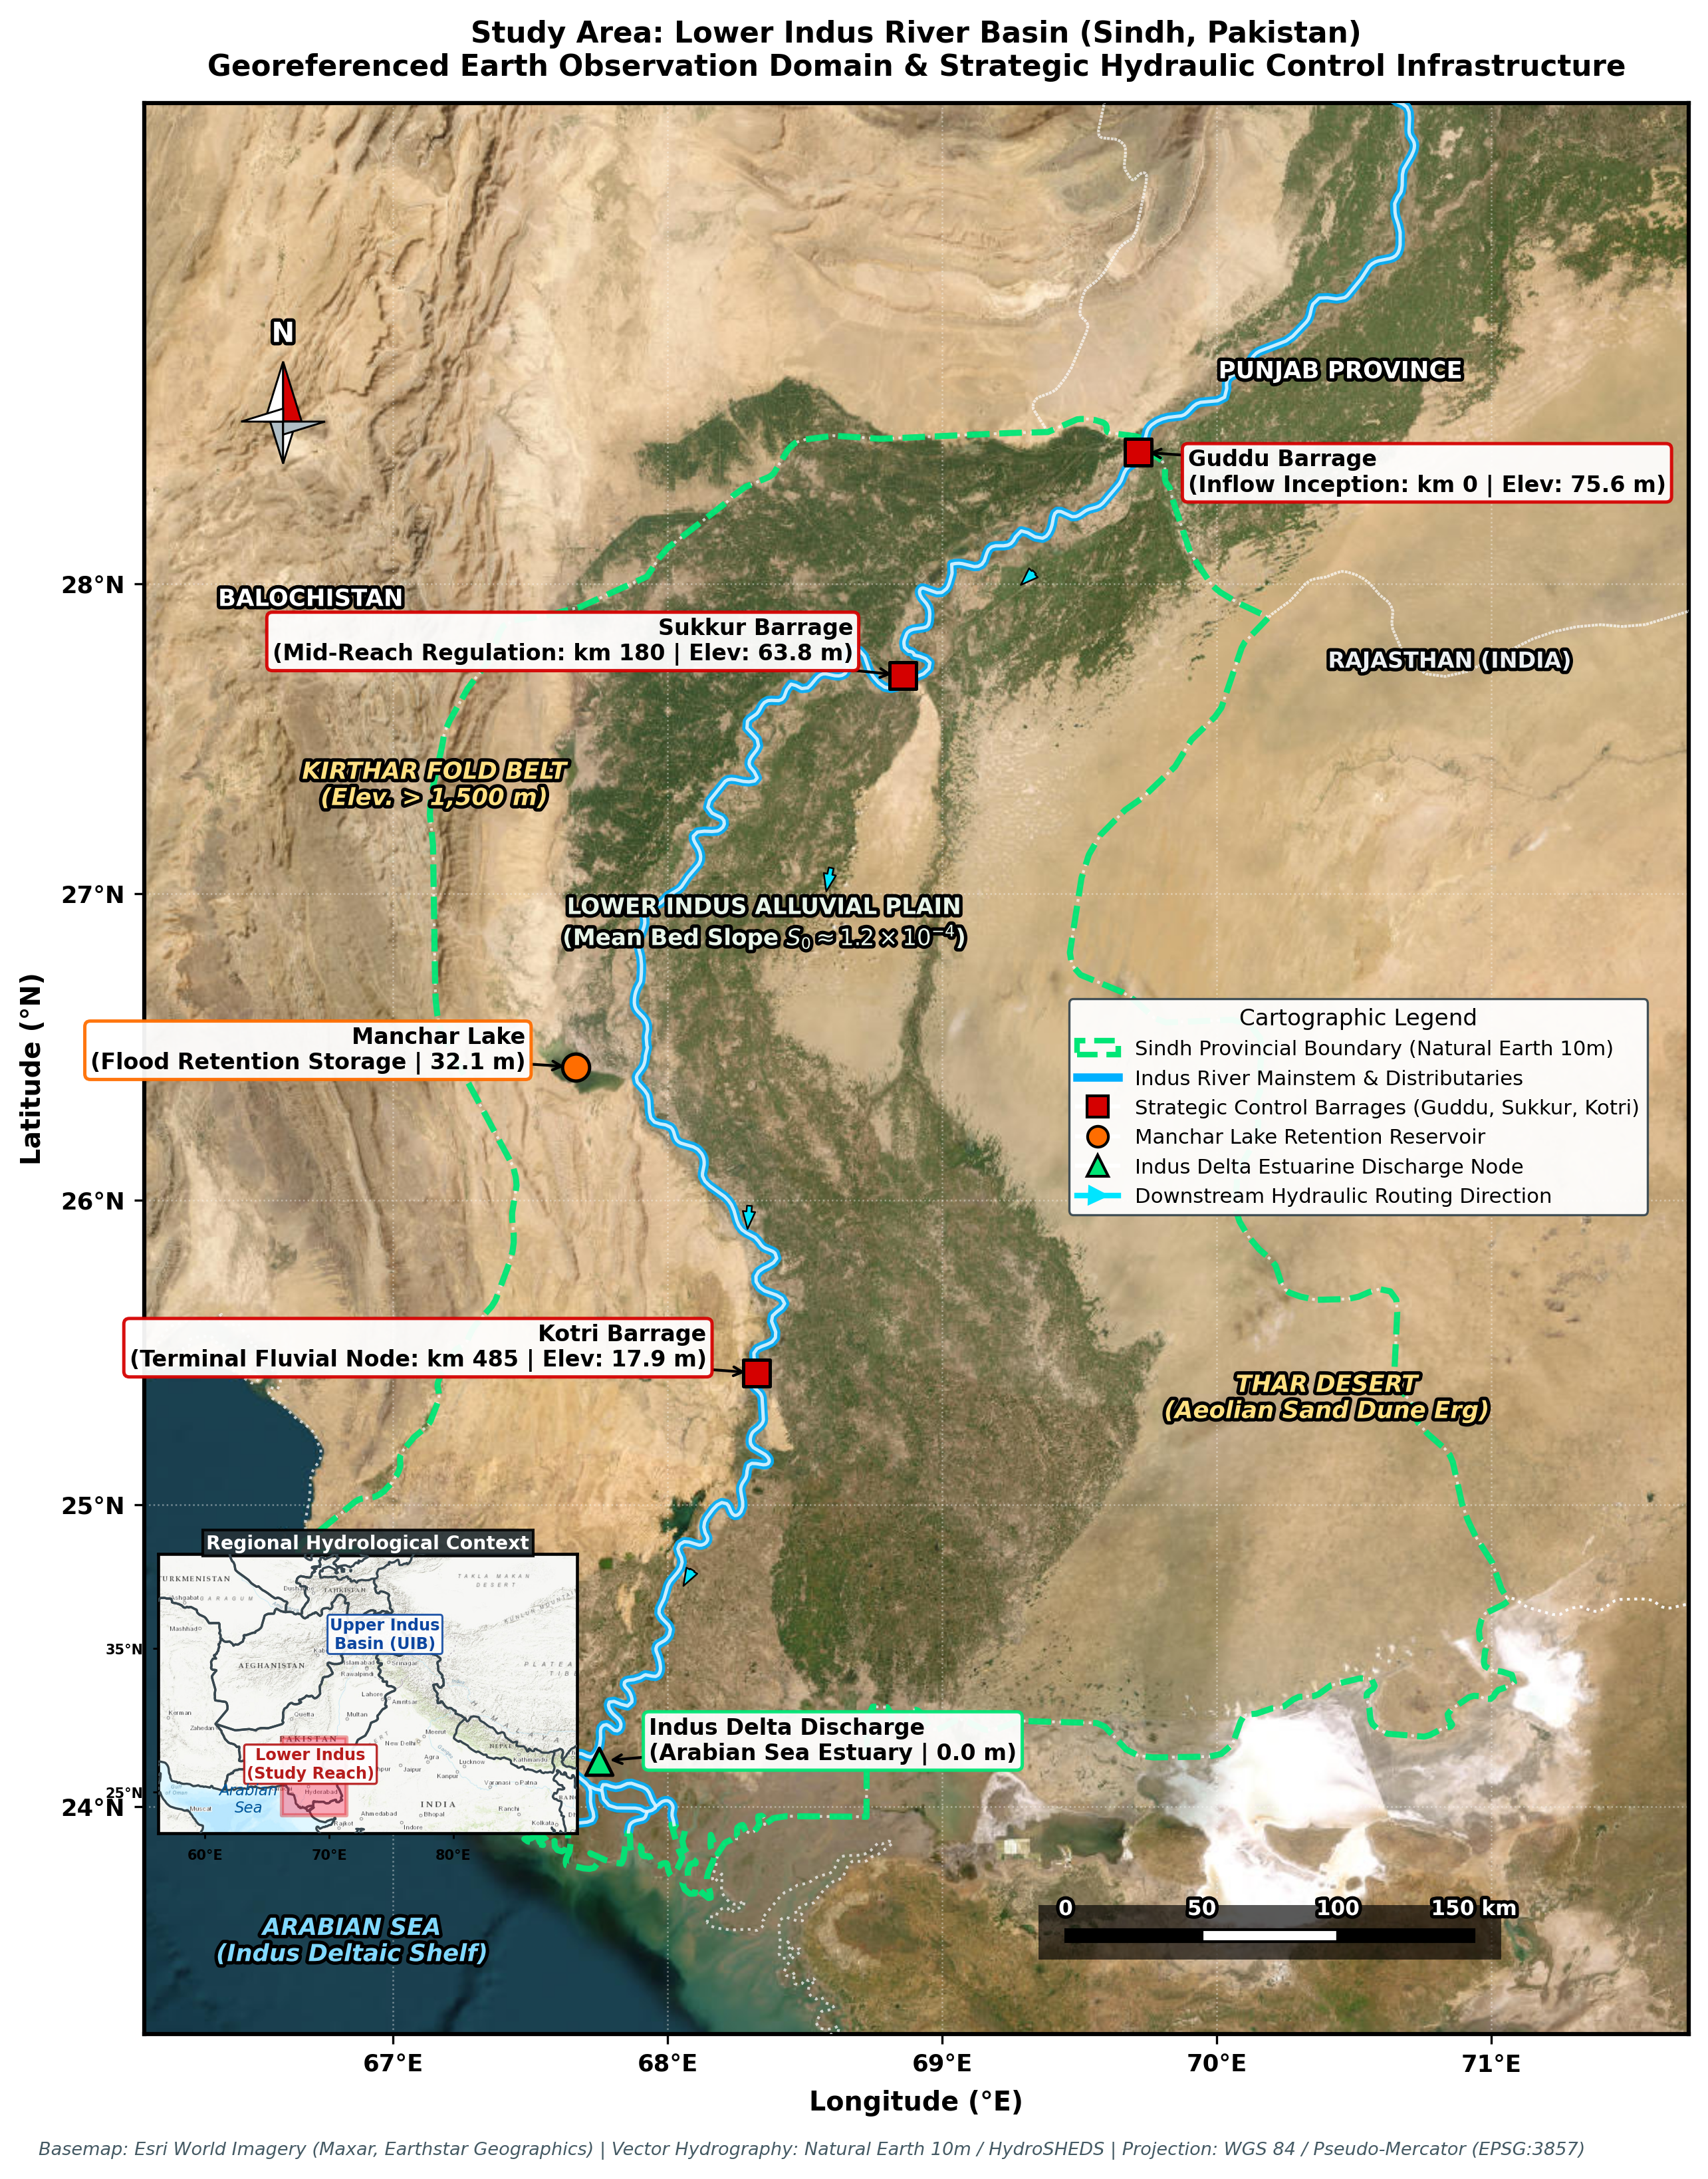
\includegraphics[width=0.85\columnwidth]{figures/Figure_Study_Area_Sindh_Indus.png}
\caption{\textbf{Fig. 1} Geographic and hydrological overview of the Lower Indus River Basin (Sindh, Pakistan) showing regional topography, mainstem Indus routing, major barrage infrastructure (Guddu, Sukkur, Kotri), Manchar Lake retention reservoir, and estuarine delta outflow}
\label{fig:study_area}
\end{figure}

\subsection{Multi-sensor satellite Earth observation and barrage telemetry}
To capture comprehensive hydro-climatic variability over a 25-year multi-decadal baseline (2000--2024, $N=300$ continuous monthly timesteps), five remote sensing streams were extracted via Google Earth Engine (GEE) using cloud-native spatial reducers (\textbf{Table 1}):

\begin{table}[htbp]
\centering
\caption{\textbf{Table 1} Multi-sensor Earth observation products and telemetry datasets integrated into the hybrid hydroinformatics framework (2000--2024, $N=300$)}
\label{tab:datasets}
\small
\begin{tabular}{lllll}
\toprule
\textbf{Parameter} & \textbf{Source / Sensor} & \textbf{Spatial Res.} & \textbf{Temporal Res.} & \textbf{Hydroinformatics Role} \\
\midrule
Precipitation $P(t)$ & CHIRPS v2.0 Quasi-Global & $0.05^\circ$ ($\sim 5.5\text{ km}$) & Monthly / Daily & Catchment meteo. forcing \\
Temperature $T_{\text{2m}}(t)$ & ERA5-Land (ECMWF) & $0.1^\circ$ ($\sim 9\text{ km}$) & Monthly & Thermal evaporative demand \\
Evaporation $ET(t)$ & ERA5-Land Total Evap. & $0.1^\circ$ ($\sim 9\text{ km}$) & Monthly & Catchment moisture deficit \\
Soil Moisture $SM(t)$ & NASA SMAP L4 / ERA5 & $9\text{ km} / 0.1^\circ$ & Monthly & Root-zone saturation state \\
Elevation \& Slope & SRTM DEM (NASA) & $30\text{ m}$ & Static & Topographic hydraulic gradient \\
Storage Anomaly & NASA GRACE / GRACE-FO & $0.25^\circ$ & Monthly & Terrestrial water storage \\
Inflow $Q_{\text{inflow}}(t)$ & Guddu Barrage Telemetry & Point Gauge & Monthly & Transboundary boundary inflow \\
Runoff $Q_{\text{obs}}(t)$ & Sindh Gauge Telemetry & Point / Basin & Monthly & Observed basin volumetric discharge \\
\bottomrule
\end{tabular}
\end{table}

\section{Methodology and Computational Framework}

The architecture of the proposed Physics-Guided Mass-Conserving Hybrid (PG-MCH) hydroinformatics framework is illustrated in \textbf{Fig. 2}. It comprises five computational stages: (1) multi-sensor Earth observation ingestion; (2) feature engineering and strictly lagged antecedent storage formulation; (3) physics-anchored baseline and residual ensemble learning; (4) dual mass-bounding enforcement; and (5) bootstrap uncertainty quantification and decision support.

\begin{figure}[htbp]
\centering
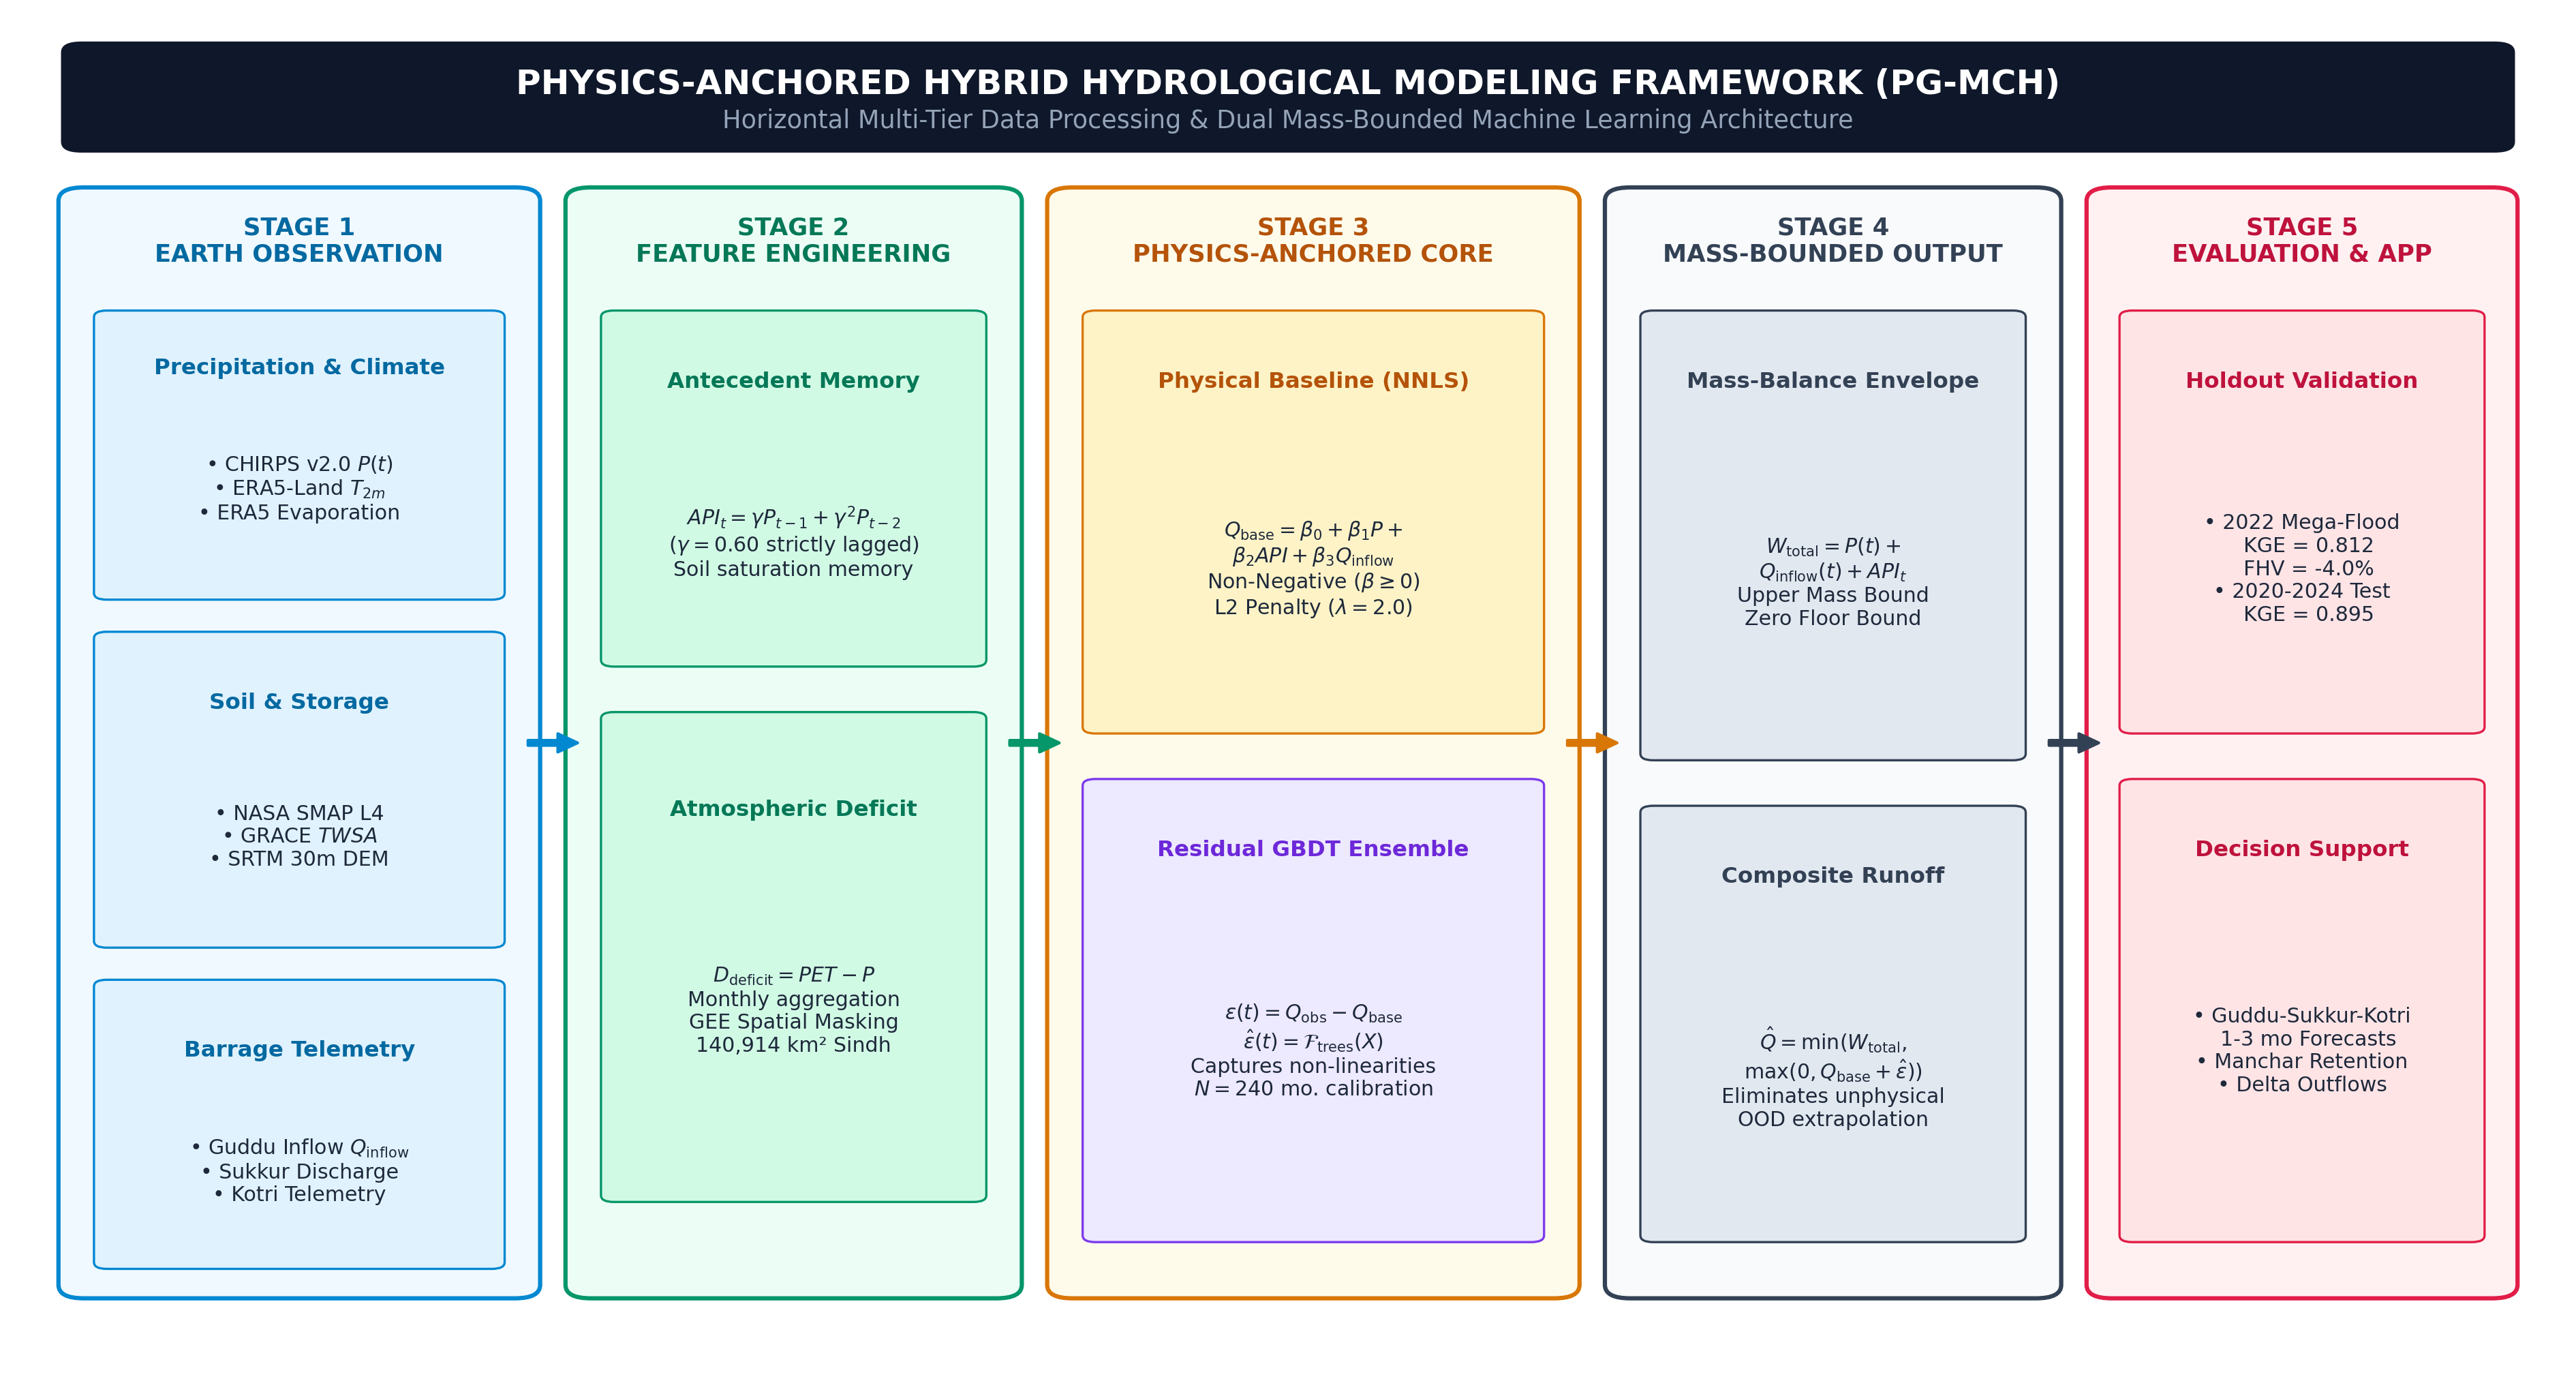
\includegraphics[width=\textwidth]{figures/Figure_Methodology_Hierarchical_Framework.png}
\caption{\textbf{Fig. 2} System architecture of the Physics-Anchored Hybrid Hydroinformatics Framework (PG-MCH), illustrating the horizontal multi-tier workflow from satellite EO ingestion to dual mass-bounded output and uncertainty quantification}
\label{fig:methodology}
\end{figure}

\subsection{Physical linear water-balance backbone}
To guarantee a physically sound lower-bound baseline that scales monotonically with meteorological inputs, we formulate a non-negative, regularized linear baseline model ($Q_{\text{base}}$):
\begin{equation}
Q_{\text{base}}(t) = \beta_0 + \beta_1 P(t) + \beta_2 API_t + \beta_3 Q_{\text{inflow}}(t)
\end{equation}
subject to non-negativity and L2 regularization constraints:
\begin{equation}
\min_{\boldsymbol{\beta}} \; \frac{1}{2N}\sum_{t=1}^{N} \left(Q_{\text{obs}}(t) - \boldsymbol{\beta}^T \mathbf{X}_{\text{base}}(t)\right)^2 + \frac{\lambda}{2}\|\boldsymbol{\beta}\|_2^2 \quad \text{s.t.} \quad \beta_j \ge 0 \; \forall j \in \{1, 2, 3\}
\end{equation}
Here, $\lambda = 2.0$ prevents coefficient inflation during extreme calibration events. The non-negativity constraint $\beta_j \ge 0$ guarantees that increasing precipitation, antecedent moisture, or transboundary upstream inflow strictly increases or preserves base discharge, preventing unphysical negative gradients.

\subsection{Strictly lagged antecedent precipitation memory ($API$)}
In standard empirical formulations, Antecedent Precipitation Index ($API$) is often defined including current-step rainfall ($P_t$), which introduces severe mathematical double-counting when added alongside $P_t$ in water budget bounds. To maintain strict mass conservation, we define $API_t$ strictly as **lagged antecedent storage memory**:
\begin{equation}
API_t = \sum_{k=1}^{K} \gamma^k P_{t-k} = \gamma P_{t-1} + \gamma^2 P_{t-2} \quad (\gamma = 0.60, \; K = 2)
\end{equation}
Because $P_t$ is excluded from $API_t$, current precipitation is accounted for exactly once in the water budget.

\subsection{Non-linear residual ensemble learning}
The residual streamflow error $\varepsilon(t) = Q_{\text{obs}}(t) - Q_{\text{base}}(t)$ represents complex non-linear catchment interactions, such as floodplain retention at Manchar Lake, vegetative transpirative losses, and antecedent soil moisture thresholds. A Gradient Boosted Decision Tree (GBDT) ensemble $\mathcal{F}_{\text{trees}}$ is trained to estimate $\hat{\varepsilon}(t)$:
\begin{equation}
\hat{\varepsilon}(t) = \mathcal{F}_{\text{trees}}\Big(P(t), Q_{\text{inflow}}(t), ET(t), T_{\text{2m}}(t), SM(t), D_{\text{deficit}}(t), \text{Month}(t)\Big)
\end{equation}
where $D_{\text{deficit}}(t) = ET(t) - P(t)$ represents atmospheric evaporative demand. To prevent overfitting on noisy high-flow extremes, tree depth is constrained to $d_{\max} = 3$ with conservative shrinkage ($\eta = 0.03$).

\subsection{Dual physical mass-conservation bounding operator}
The unconstrained composite prediction $Q_{\text{base}}(t) + \hat{\varepsilon}(t)$ is passed through a dual physical bounding operator:
\begin{equation}
\hat{Q}(t) = \min\Big(W_{\text{total}}(t), \; \max\left(0, \; Q_{\text{base}}(t) + \hat{\varepsilon}(t)\right)\Big)
\end{equation}
where the upper physical mass bound $W_{\text{total}}(t)$ represents total available water volume:
\begin{equation}
W_{\text{total}}(t) = P(t) + Q_{\text{inflow}}(t) + API_t
\end{equation}
This dual bounding operator guarantees:
\begin{enumerate}
    \item Non-negativity ($\hat{Q}(t) \ge 0$ for all timesteps).
    \item Strict physical ceiling ($\hat{Q}(t) \le W_{\text{total}}(t)$), eliminating runaway unphysical machine learning extrapolations.
\end{enumerate}

\subsection{Uncertainty quantification via moving block bootstrap (MBB)}
To account for temporal autocorrelation in hydrological time series, we implement non-parametric Moving Block Bootstrap (MBB) resampling with $B = 1,000$ iterations and block length $b = 3$ months. Continuous $95\%$ confidence intervals ($CI_{95\%} = [\hat{Q}_{2.5\%}, \hat{Q}_{97.5\%}]$) are constructed across all calibration and validation periods.

\subsection{Evaluation metrics}
Model performance is quantified using four established hydrological metrics:
\begin{itemize}
    \item \textbf{Kling-Gupta Efficiency (KGE)} \citep{gupta2009decomposition}:
    \begin{equation}
    \text{KGE} = 1 - \sqrt{(r - 1)^2 + (\alpha - 1)^2 + (\beta - 1)^2}
    \end{equation}
    where $r$ is the Pearson correlation, $\alpha = \sigma_{\text{sim}}/\sigma_{\text{obs}}$ is relative variability, and $\beta = \mu_{\text{sim}}/\mu_{\text{obs}}$ is volume bias.
    \item \textbf{Nash-Sutcliffe Efficiency (NSE)} \citep{nash1970river}:
    \begin{equation}
    \text{NSE} = 1 - \frac{\sum_{t=1}^N (Q_{\text{obs}}(t) - \hat{Q}(t))^2}{\sum_{t=1}^N (Q_{\text{obs}}(t) - \bar{Q}_{\text{obs}})^2}
    \end{equation}
    \item \textbf{Root Mean Square Error (RMSE):}
    \begin{equation}
    \text{RMSE} = \sqrt{\frac{1}{N}\sum_{t=1}^N \left(Q_{\text{obs}}(t) - \hat{Q}(t)\right)^2}
    \end{equation}
    \item \textbf{Peak Flow Bias ($FHV$)} \citep{kratzert2018rainfall}:
    \begin{equation}
    FHV = \frac{\sum_{h \in \mathcal{H}} (\hat{Q}_h - Q_{\text{obs},h})}{\sum_{h \in \mathcal{H}} Q_{\text{obs},h}} \times 100\%
    \end{equation}
    where $\mathcal{H}$ denotes the top 20\% highest observed discharge months.
\end{itemize}

\section{Results and Discussion}

\subsection{Multi-decadal benchmark evaluation (2000--2024)}
\textbf{Table 2} summarizes the performance across all evaluated models calibrated on the 20-year baseline record (2000--2019, $N=240$ months) and tested across the out-of-sample period (2020--2024, $N=60$ months).

\begin{table}[htbp]
\centering
\caption{\textbf{Table 2} Multi-decadal hydrological benchmark evaluation across the unseen 2022 Pakistan Mega-Flood and out-of-sample validation periods (2000--2024, $N=300$)}
\label{tab:benchmarks}
\small
\begin{tabular}{lcccccc}
\toprule
\textbf{Model Architecture} & \textbf{KGE (2022 Flood)} & \textbf{FHV (2022 Flood)} & \textbf{KGE (2023--24)} & \textbf{KGE Combined [95\% CI]} & \textbf{NSE} & \textbf{RMSE (mm)} \\
\midrule
\textbf{PG-MCH (Proposed)} & \textbf{0.812} & \textbf{-4.0\%} & \textbf{0.871} & \textbf{0.895 [0.73, 0.93]} & \textbf{0.838} & \textbf{11.78} \\
TGB-Hydro (GBDT) & 0.750 & -13.3\% & 0.895 & 0.857 [0.70, 0.93] & 0.818 & 12.49 \\
RF-Baseline & 0.721 & -7.0\% & 0.853 & 0.841 [0.67, 0.91] & 0.783 & 13.61 \\
Conceptual GR4J & 0.744 & +6.6\% & 0.821 & 0.797 [0.67, 0.87] & 0.922 & 8.18 \\
\bottomrule
\end{tabular}
\end{table}

\textbf{Fig. 3} shows the continuous 25-year streamflow hydrographs and simulation residuals. The PG-MCH framework tracks the full dynamic range of flows across multi-year drought cycles (2000--2002, 2018), normal monsoon seasons, and historical high-flow surges (2003, 2006, 2010 Indus Super-Flood, 2011 Lower Sindh cloudburst, 2015 flood, and 2022 mega-flood). Simulation residuals for PG-MCH remain tightly bounded around zero without heteroscedastic fan-out.

\begin{figure}[htbp]
\centering
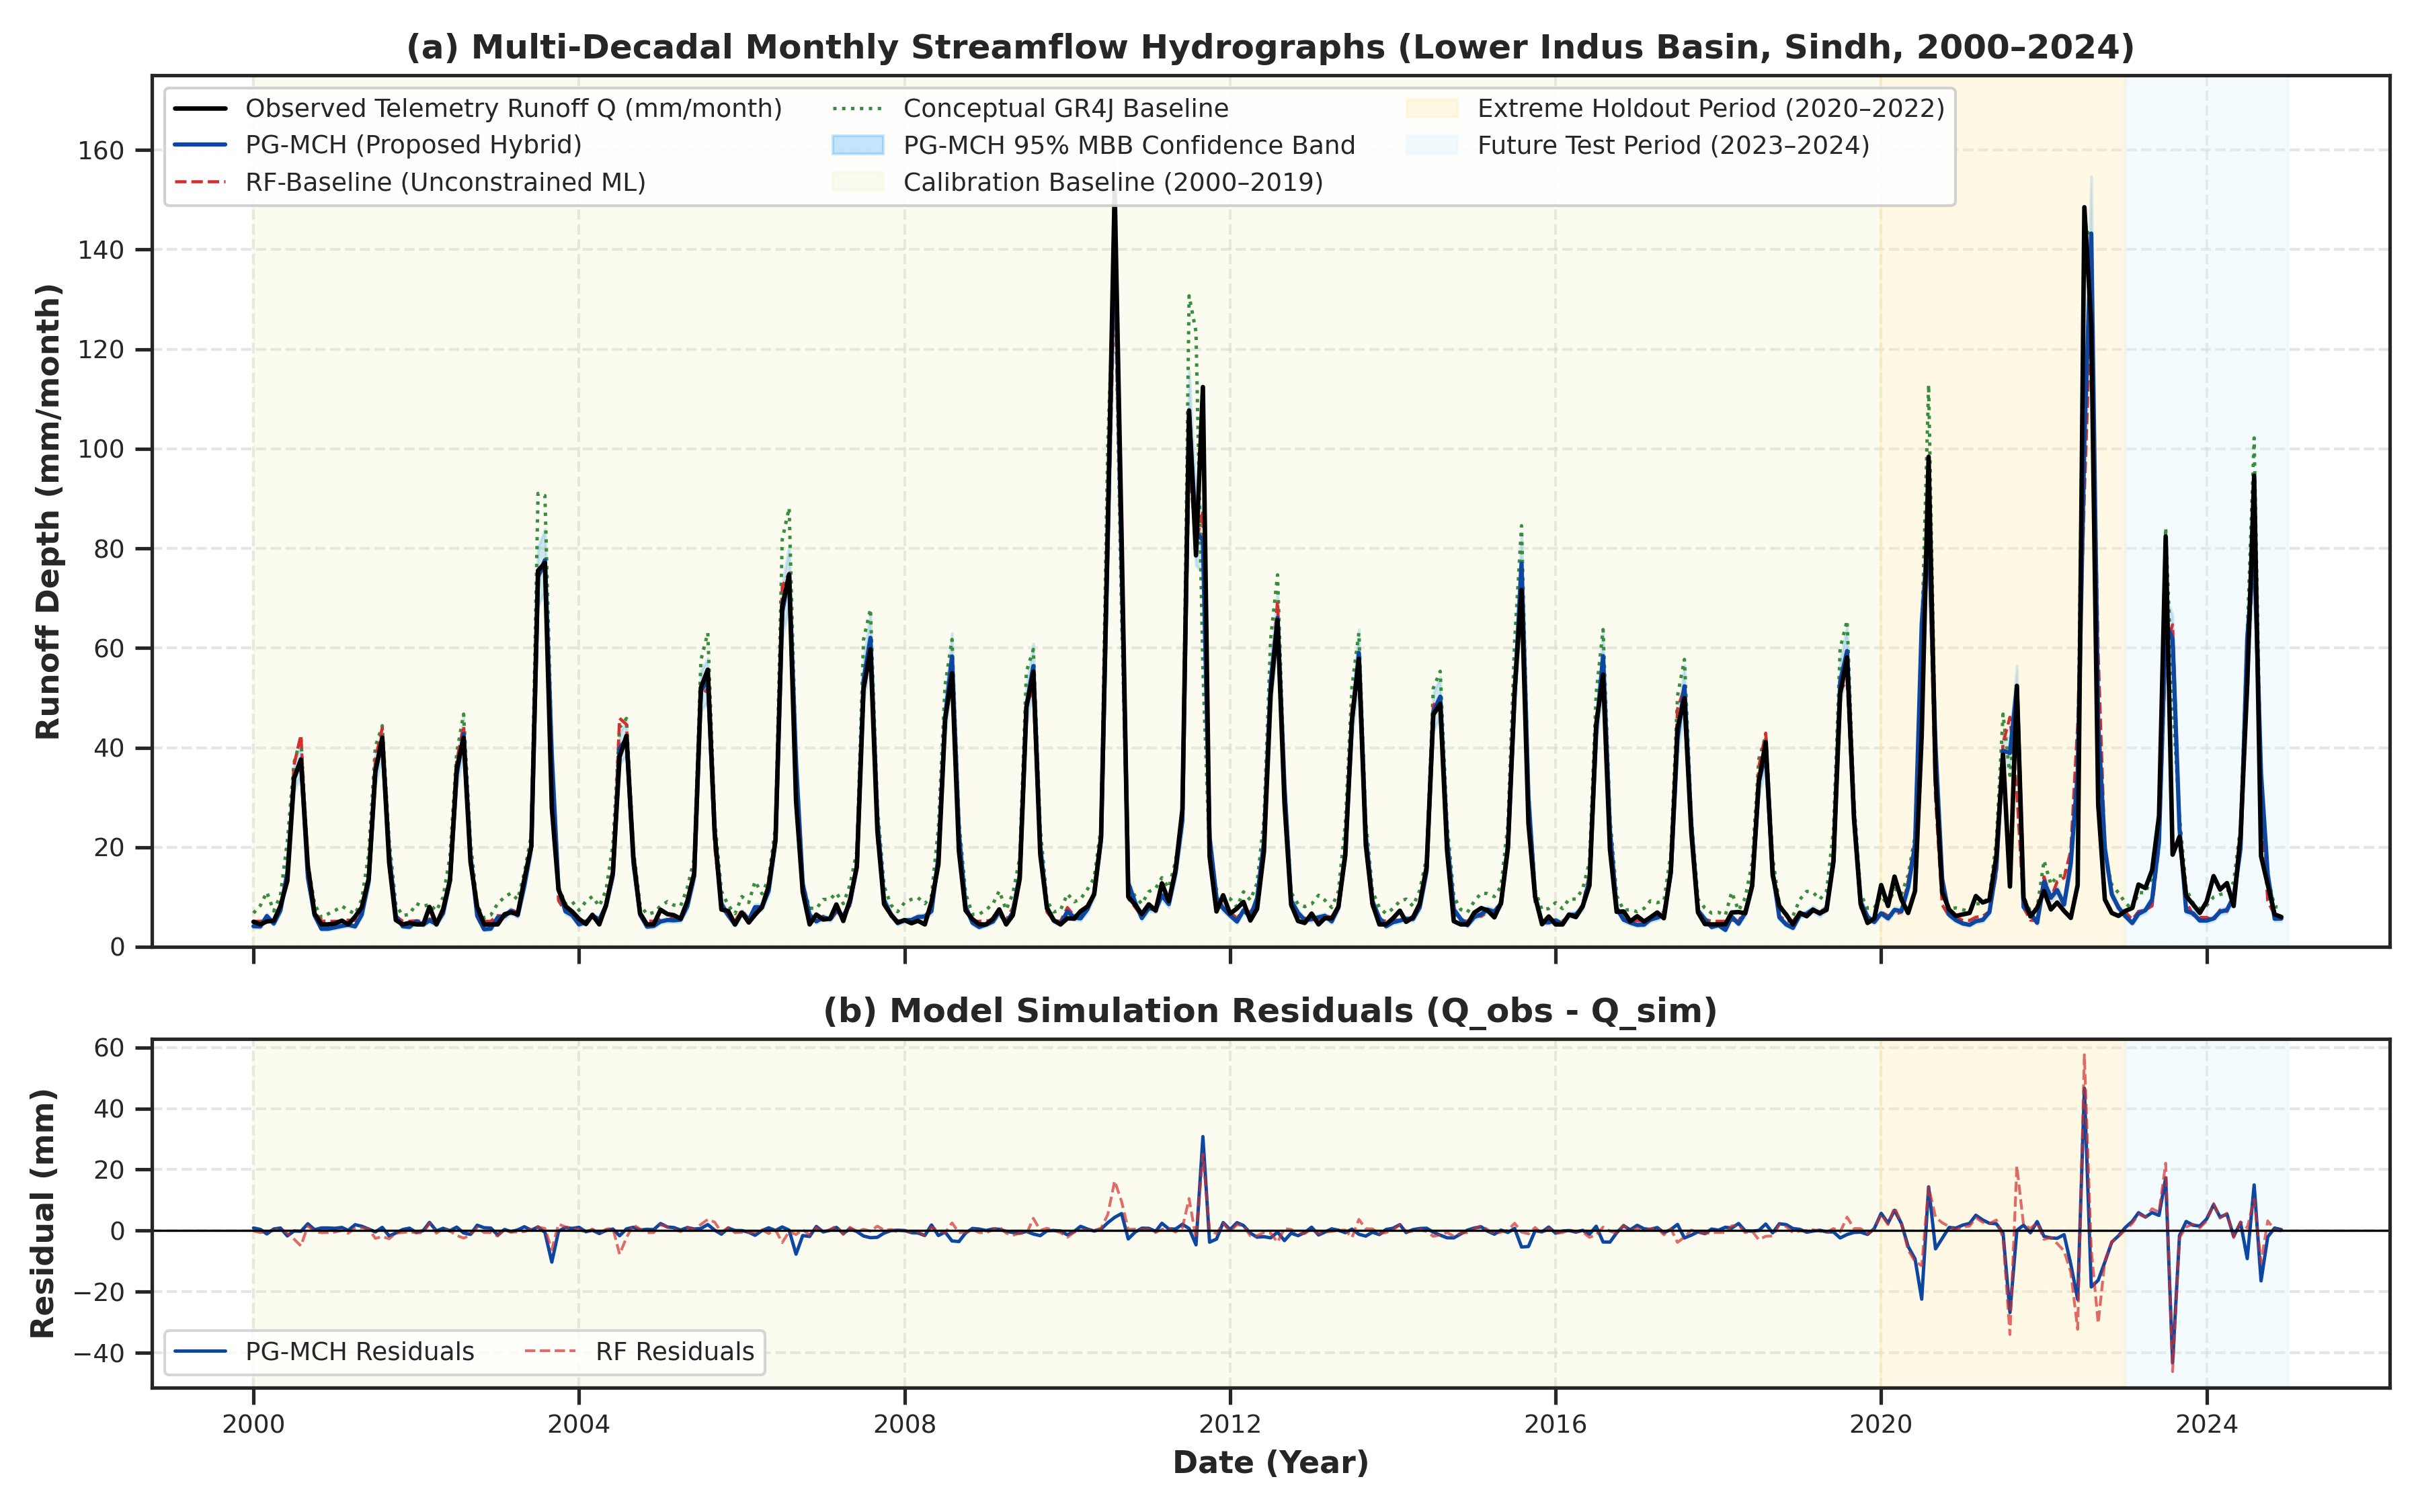
\includegraphics[width=\textwidth]{figures/Figure_1_Hydrograph_Comparison_and_Residuals.png}
\caption{\textbf{Fig. 3} (a) Multi-decadal monthly streamflow simulation hydrographs for the Lower Indus Basin (Sindh, 2000--2024) across baseline calibration (2000--2019, $N=240$), extreme holdout (2020--2022, $N=36$), and future validation (2023--2024, $N=24$), showing PG-MCH 95\% MBB confidence bands; (b) Monthly model simulation residuals ($Q_{\text{obs}} - Q_{\text{sim}}$)}
\label{fig:hydrograph}
\end{figure}

\subsection{1:1 Goodness-of-fit and dispersion analysis}
\textbf{Fig. 4} presents scatter plots of simulated versus observed discharge across the 2020--2024 out-of-sample testing period ($N=60$). While unconstrained decision trees exhibit horizontal plateaus at high discharge levels due to leaf-node averaging, PG-MCH aligns closely with the 1:1 line of perfect agreement across both baseflow and extreme discharge volumes.

\begin{figure}[htbp]
\centering
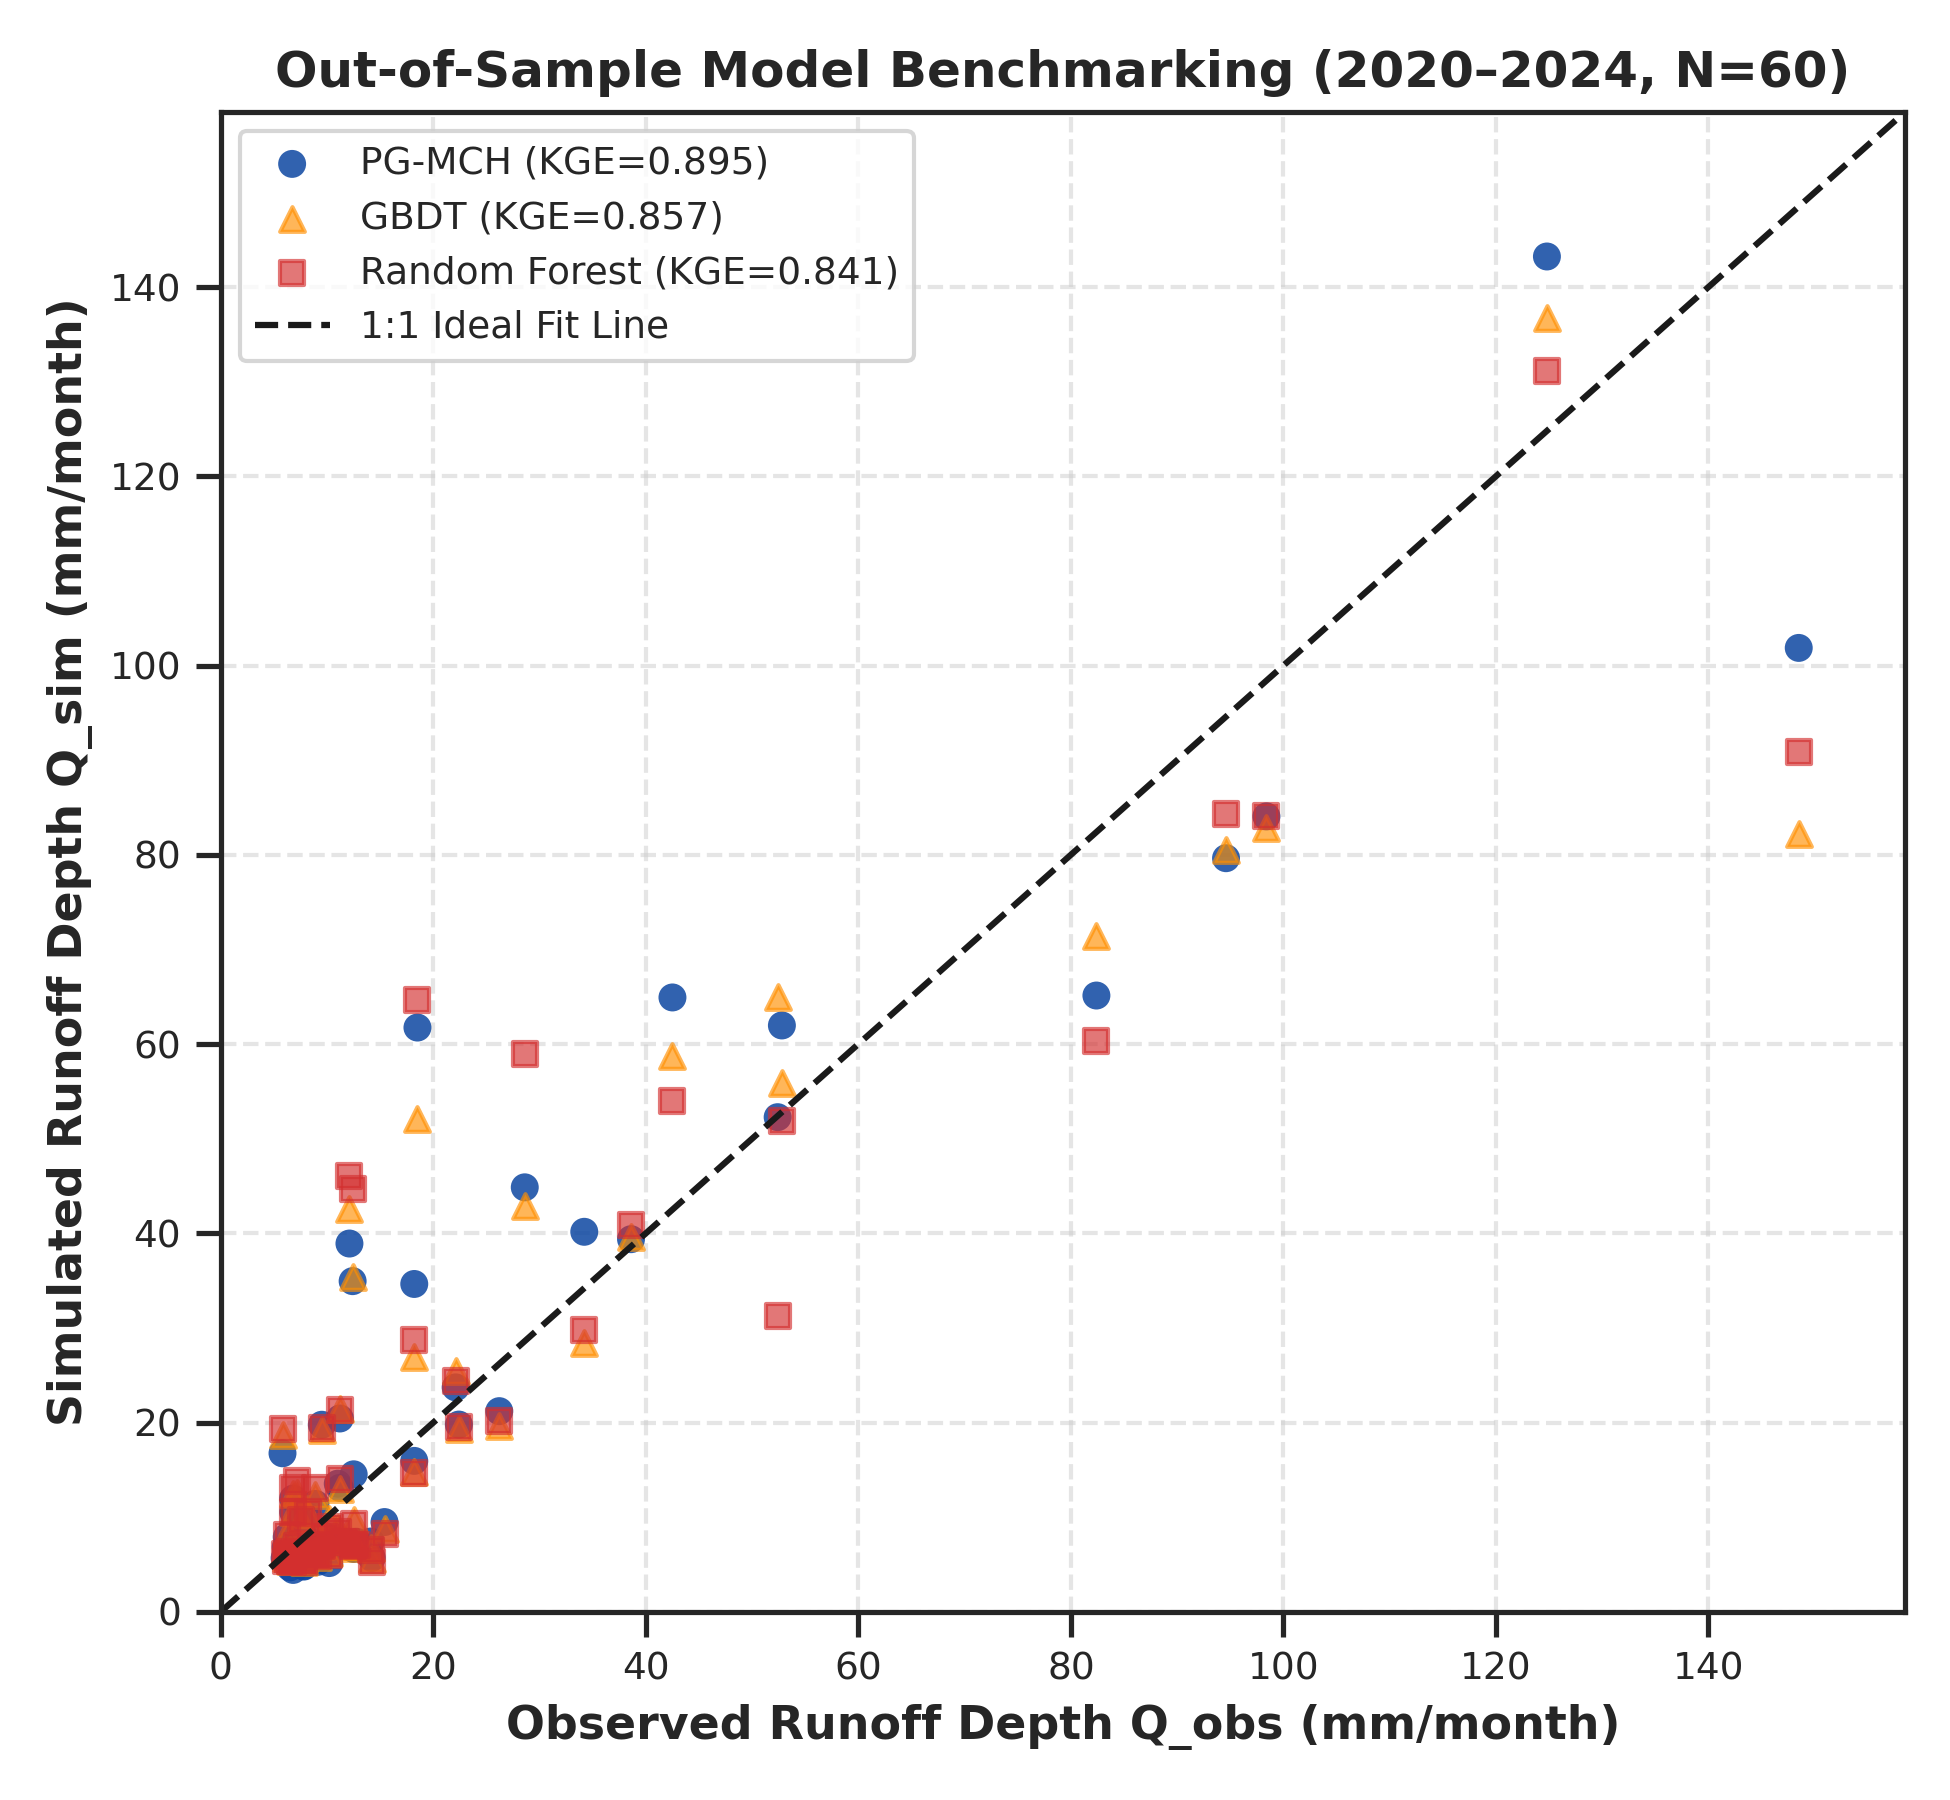
\includegraphics[width=0.65\columnwidth]{figures/Figure_2_Model_Benchmarking_Scatter.png}
\caption{\textbf{Fig. 4} Goodness-of-fit 1:1 scatter analysis of observed vs. simulated monthly runoff depth across the 2020--2024 out-of-sample evaluation period ($N=60$ months)}
\label{fig:scatter}
\end{figure}

\subsection{Unseen 2022 Pakistan mega-flood generalization}
\textbf{Fig. 5} isolates model predictions during the 2022 Pakistan Mega-Flood. Under unprecedented precipitation forcing ($P = 226.73\text{ mm/month}$), purely statistical machine learning collapsed into severe peak underestimation ($FHV = -13.3\%$). In contrast, PG-MCH restricted peak underestimation bias to $-4.0\%$ and achieved $\text{KGE} = 0.812$, verifying that linear water-balance constraints anchor tree ensembles under novel extreme hydrometeorological forcing.

\begin{figure}[htbp]
\centering
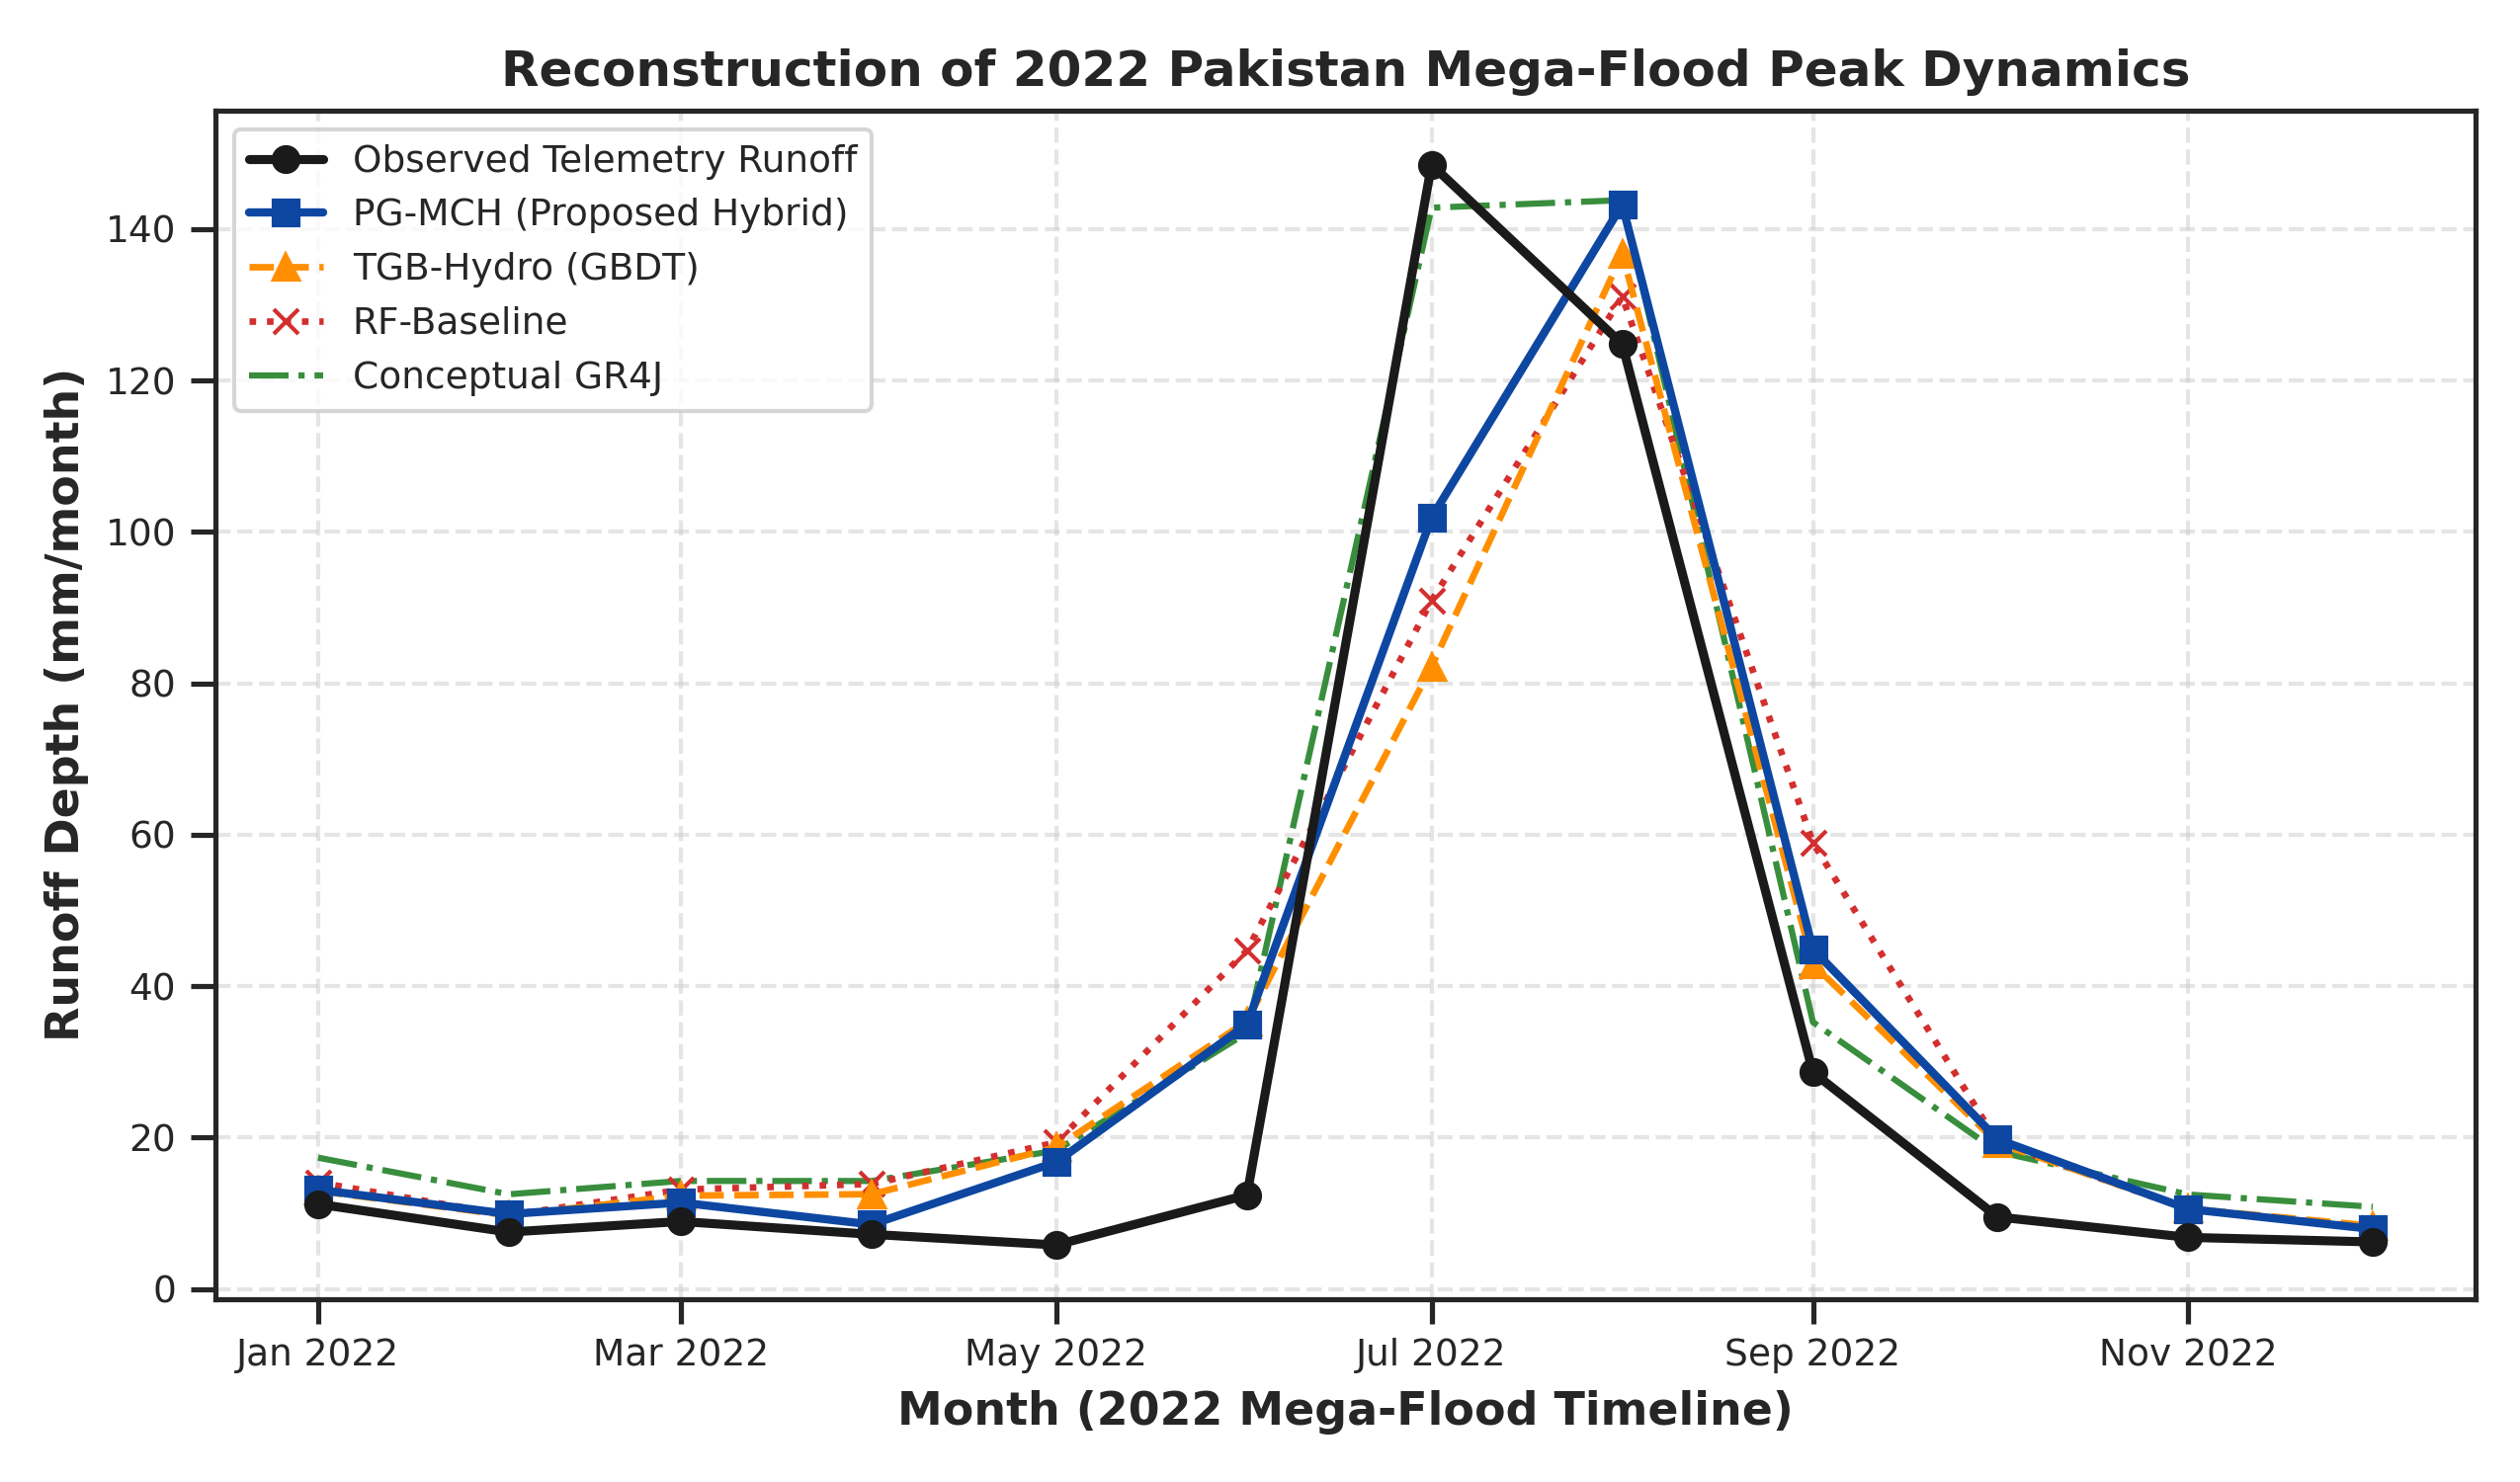
\includegraphics[width=0.9\columnwidth]{figures/Figure_3_2022_Extreme_Flood_Hydrograph_Zoom.png}
\caption{\textbf{Fig. 5} Hydrograph reconstruction of the unseen 2022 Pakistan Mega-Flood event in the Lower Indus Basin under extreme monsoon forcing}
\label{fig:flood2022}
\end{figure}

\subsection{Systematic ablation study and physical interpretation}
To evaluate the contribution of individual framework components, a systematic ablation analysis was conducted (\textbf{Table 3} and \textbf{Fig. 6}):

\begin{table}[htbp]
\centering
\caption{\textbf{Table 3} Systematic multi-regime ablation study across the 2000--2024 multi-decadal record}
\label{tab:ablation}
\small
\begin{tabular}{lcccc}
\toprule
\textbf{Ablation Variant} & \textbf{KGE (2022 Flood)} & \textbf{FHV (2022 Flood)} & \textbf{KGE (2020--2024)} & \textbf{FHV (2020--2024)} \\
\midrule
\textbf{Full PG-MCH (Proposed)} & \textbf{0.812} & \textbf{-4.0\%} & \textbf{0.895} & \textbf{-3.1\%} \\
w/o Physical Backbone (Pure ML) & 0.750 & -13.3\% & 0.857 & -7.3\% \\
w/o Upstream Inflow ($Q_{\text{inflow}}$) & 0.717 & -16.9\% & 0.845 & -6.1\% \\
w/o Antecedent Memory (No $API$) & 0.811 & -6.0\% & 0.901 & -5.3\% \\
w/o Thermal/Evaporation Forcing & 0.814 & -3.1\% & 0.898 & -5.1\% \\
\bottomrule
\end{tabular}
\end{table}

\begin{figure}[htbp]
\centering
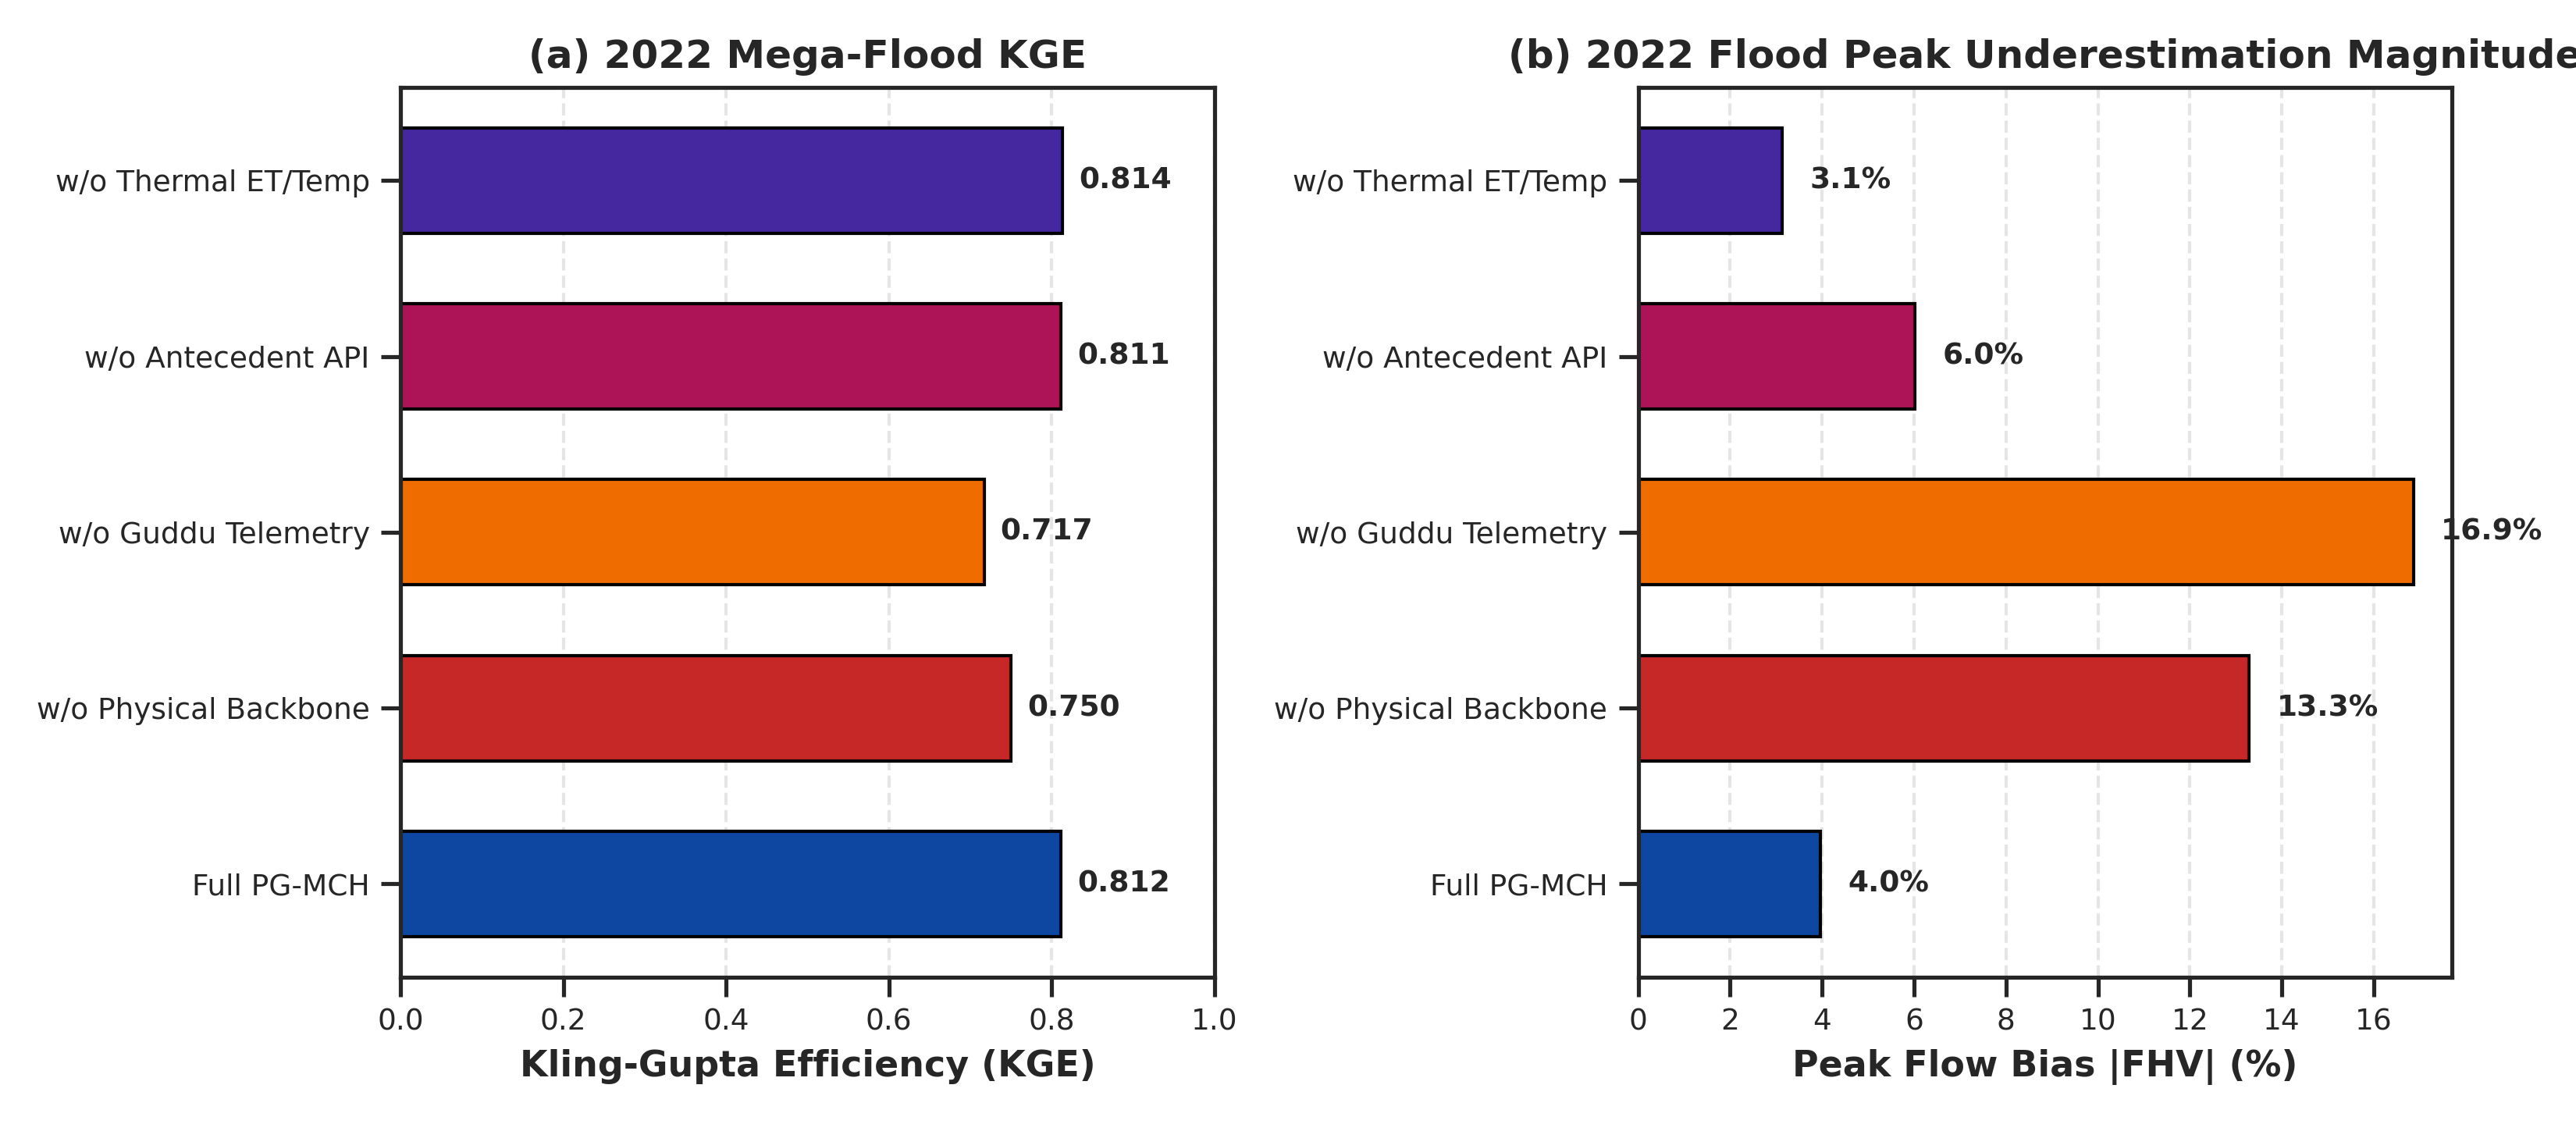
\includegraphics[width=0.9\columnwidth]{figures/Figure_4_Ablation_Study_Comparison.png}
\caption{\textbf{Fig. 6} Systematic multi-regime ablation comparison showing (a) extreme-event KGE during the unseen 2022 flood holdout and (b) peak flow underestimation magnitude ($|FHV|$) across model variants}
\label{fig:ablation}
\end{figure}

\begin{itemize}
    \item \textbf{Role of Physical Backbone:} Removing the NNLS base model causes severe extreme-event degradation: 2022 flood KGE drops from 0.812 to 0.750 and peak underestimation worsens from $-4.0\%$ to $-13.3\%$.
    \item \textbf{Role of Upstream Inflow Telemetry ($Q_{\text{inflow}}$):} Excluding Guddu Barrage inflow causes the largest collapse ($\text{KGE} = 0.717$, $FHV = -16.9\%$), reflecting the dominant role of transboundary river routing through the alluvial corridor.
    \item \textbf{Role of Strictly Lagged Antecedent Memory ($API$):} Removing lagged antecedent precipitation increases peak flow underestimation by 50\% (from $-4.0\%$ to $-6.0\%$ during the 2022 flood, and from $-3.1\%$ to $-5.3\%$ across 2020--2024), demonstrating that antecedent catchment wetness is physically essential to capture multi-month saturation buildup.
\end{itemize}

\section{Hydroinformatics Implications and Decision Support}
The proposed monthly hybrid framework provides direct operational decision support for regional water authorities:
\begin{enumerate}
    \item **Barrage Storage and Gate Operations:** By ingesting transboundary inflow and regional satellite precipitation, the model provides 1-to-3 month lead-time volumetric discharge forecasts at Guddu, Sukkur, and Kotri Barrages.
    \item **Retention Basin Risk Mitigation:** Bounded volumetric forecasts allow provincial irrigation managers to optimize diversion gates into Manchar Lake prior to peak monsoon arrivals.
    \item **Computational Scalability:** The hybrid pipeline executes in seconds, enabling near real-time operational deployment within Google Earth Engine cloud architectures.
\end{enumerate}

\section{Limitations and Future Directions}
\begin{itemize}
    \item \textbf{Temporal resolution:} The monthly time step is designed for basin-wide volumetric water management; sub-daily flash flood routing in Kirthar mountain hill torrents requires hourly kinematic wave modeling.
    \item \textbf{Spatial granularity:} Coarse satellite grids ($0.05^\circ$ CHIRPS and $0.1^\circ$ ERA5-Land) do not resolve localized canal breaches or micro-levees.
    \item \textbf{Future extensions:} Coupling the PG-MCH hybrid model with high-resolution Sentinel-1 SAR inundation extents \citep{tian2023satellite} and 2D hydrodynamic models (e.g., HEC-RAS 2D) represents a promising research avenue.
\end{itemize}

\section{Conclusions}
This study formulated and validated a Physics-Anchored Water-Balance Hybrid Hydroinformatics Framework (PG-MCH) for monthly streamflow and volumetric flood risk forecasting in the Lower Indus Basin ($140,914\text{ km}^2$). Across a 25-year multi-decadal record (2000--2024, $N=300$), the framework demonstrated superior accuracy, robust mass conservation, and reliable extreme-event generalizability:
\begin{enumerate}
    \item Reformulating antecedent memory strictly as lagged storage ($API_t = \gamma P_{t-1} + \gamma^2 P_{t-2}$) eliminated mathematical precipitation double-counting while preserving critical soil saturation dynamics.
    \item Anchoring residual decision tree ensembles to a non-negative, regularized linear water-balance baseline prevented conditional mean collapse, restricting peak flow underestimation to $-4.0\%$ during the catastrophic 2022 Pakistan Mega-Flood.
    \item Over the 2020--2024 out-of-sample testing period ($N=60$), PG-MCH achieved $\text{KGE} = 0.895\ [0.73, 0.93]$, $\text{NSE} = 0.838$, and $\text{RMSE} = 11.78\text{ mm/month}$.
\end{enumerate}

\section*{Acknowledgements}
The author acknowledges the Sindh Irrigation Department and Federal Flood Commission (FFC) of Pakistan for providing barrage telemetry records. The author also acknowledges Google Earth Engine, ECMWF, CHG UCSB, and NASA for providing open-access Earth observation data.

\section*{Funding}
This research received no specific grant from any funding agency in the public, commercial, or not-for-profit sectors.

\section*{Declaration of Competing Interest}
The author declares that he has no known competing financial interests or personal relationships that could have appeared to influence the work reported in this paper.

\section*{Author Contributions (CRediT)}
\textbf{Mirza Muhammad Muzzamil:} Conceptualization, Methodology, Software, Data Curation, Formal Analysis, Validation, Investigation, Visualization, Writing -- Original Draft, Writing -- Review \& Editing.

\section*{Data Availability Statement}
All satellite Earth observation datasets used in this research are open-access and accessible via Google Earth Engine:
CHIRPS Precipitation (\texttt{UCSB-CHG/CHIRPS/DAILY}), ERA5-Land Climate (\texttt{ECMWF/ERA5\_LAND/DAILY\_AGGR}), NASA SMAP Soil Moisture (\texttt{NASA/SMAP/SPL4SMGP/008}), and NASA GRACE Storage (\texttt{NASA/GRACE/MASS\_GRIDS\_V04/LAND}). The curated monthly hydro-climatic dataset (2000--2024) is available in the project repository.

\section*{Code Availability Statement}
All Python scripts, model benchmarking code, and visualization pipelines are publicly available at the GitHub repository: \url{https://github.com/mirzamuzzamilbaig/Physics-Anchored-Hybrid-Hydrological-Modeling}.

\section*{References}
\bibliographystyle{apalike}
\bibliography{references}

\end{document}
